% ---------------------------------------------------------------------------
\section{Writing Katakana Letters}\jsec{片仮名を一つづつ書く} 
% [o] LABEL
\label{sec:WritingKatakanaLetters}
% [o] INDEX
% DESTINATION (DEF)
\ifor{Katakana}{片仮名}{かたかな}{Katakana} % TARGET

Writing \textit{Katakana words} start with writing single \textit{Katakana
letters}. Knowing the writing and reading of \textit{Katakana letters} is
essential to pronounce foreign words in Japanese correctly. And that is even
more important for learners who have good English knowledge, because it is very
tempting to pronounce English words in Japanese with original English
pronunciation, which is seldom understood\footnote{The reader might try to
order a cheeseburger at a fast food restaurant insted of a /chiizubaagaa/
(チーズバーガー).} by Japanese people who are used to their Japanese-English
pronunciation. 

By learning \textit{Katakana} the understanding of morae and syllables will
also help to improve the pronunciation and understanding of Japanese. 

\textit{Katakana} as most letters are a joint combination of strokes. For the
writing of \textit{Katakana} some rules are important, which are presented here
out of order.


\begin{description}

\item[Order:] The order of strokes is important. In section
\ref{sec:StrokeOrderMatter} on page \pageref{sec:StrokeOrderMatter} more can be
found. 

\item[Fasted Method of Writing:] Often the fastest possible method of writing
or order of strokes is the correct one.  Often from left upper corner to right
lower corner. But exceptions do exist.

\item[The characters (letters) are \textit{not} symmetric.]

\item[All characters (letters) occupy a square.]

\item[The aesthetic:] What make the character to a beautiful character? The
answer is different for each character.

Following some possibilities of rule generation for the character ``u''
 {「ウ」 }:

\bigskip \CharacterExplanation{u-guide2}{The most important feature is that the
second and third line do not align. This is not an accident.}

\bigskip \CharacterExplanation{u-guide0}{Except many
\hyperref[sec:Hiragana]{Hiragana} for some \textit{Katakana} the base line is
aligned with horizon. As with this character. }


\bigskip \CharacterExplanation{u-guide1}{Also the start (or turning) points of
all other lines are aligned vertically. Which gives this \textit{Katakana} its
unique square look.}


\bigskip \CharacterExplanation{u-guide}{All together some lines need to be
remembered to write the letter beautiful.}

\bigskip

\item[A different logic:] A little bit less the
\hyperref[sec:Hiragana]{Hiragana}, but also in \textit{Katakana} there are some
lines that do not align horizontally  or vertically. Or to say it differently
some characters are not straight on purpose.

\end{description}

On top of this the following is most likely valid: only if one can write a
letter it is (easier) possible to learn faster and memorize it.


%----------------------------------------------------------------------------
\subsection{Stroke Order Matter!}\jsubsec{書き順事項}
% [o[ LABEL 
\label{sec:StrokeOrderMatter}
% [o] INDEX

Some European individualists might ask themselves \textit{"Why do I have to
remember the order of strokes - I don't obay this in my language - and who
defined this in the first place (if not me)?"} and this seems obvious in
Europe. However some reason for order exist. 

% 書き順事項 【かきじゅんじこう】

\begin{description}

\item[1. Impression:] it makes an unprofessional impression to Japanese, if one
writes characters in the wrong order. Some laughs can be observed at least.

\item[2. Tests:]  in some tests/exams (in Japan) the order of strokes will be
tested and one gets 0 points for the wrong order. 

\item[3. Time Savings:] In the most cases the predefined order is the fastest
way to write a character. Overall once save (life) time.

\item[4. Readability:] in some cases characters become readable only (or
beautiful) if the order is correct.

\item[5. Confusion Danger:] for some characters, the order is utmost
important. If not obeyed it is very likely (ie, almost certain) that these
characters become a candidate for wrong interpretation. 

\end{description}
\normalsize

\newpage
%----------------------------------------------------------------------------
\subsection{Example /u/ }\jsubsec{{「ウ」の例} }
% [o] LABEL
\label{subsec:ExampleU}
% [o] INDEX

The \textit{Katakana} /u/ is written as {「ウ」} in Japanese. The character is
composed out of the following three components:

\bigskip 
\CharacterExplanation{uds1}{This is stroke 1}
\bigskip 
\CharacterExplanation{uds2}{This is stroke 2}
\bigskip 
\CharacterExplanation{uds3}{This is stroke 3} 

Of course the strokes need to be at the right place. So better always think or
draw a frame aound. Or even better write the strokes into a frame from the
beginning!

\bigskip 
\CharacterExplanation{udss1}{This is stroke 1 in a square frame}
\bigskip 
\CharacterExplanation{udss2}{This is stroke 2 in a square frame}
\bigskip 
\CharacterExplanation{udss3}{This is stroke 3 in a square frame} 


%\begin{center}
%\textbf{Stroke 1:} 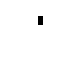
\includegraphics[trim= 00 15 00 00]{../share/katakana/uds1.pdf}
%\textbf{Stroke 2:} 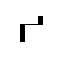
\includegraphics[trim= 00 15 00 00]{../share/katakana/uds2.pdf}
%\textbf{Stroke 3:} 
\includegraphics[trim= 00 15 00 00]{../share/katakana/uds3.pdf}
%\end{center}
\bigskip

This components have to be written in the above mentioned enumeration order one
after another. (The first example is without frame)

\bigskip 
\CharacterExplanation{udg1}{This is stroke 1 in context}
\bigskip 
\CharacterExplanation{udg2}{This is stroke 2 in context}
\bigskip 
\CharacterExplanation{udg3}{This is stroke 3 in context}

%\begin{center}
%\textbf{Stroke 1:} 
\includegraphics[trim= 00 15 00 00]{../share/katakana/udg1.pdf}
%
%\textbf{Stroke 2:} 
\includegraphics[trim= 00 15 00 00]{../share/katakana/udg2.pdf}
%
%\textbf{Stroke 3:} 
\includegraphics[trim= 00 15 00 00]{../share/katakana/udg3.pdf}
%\end{center}

\bigskip 
\CharacterExplanation{udgs1}{This is stroke 1 in context in a square frame}
\bigskip 
\CharacterExplanation{udgs2}{This is stroke 2 in context in a square frame}
\bigskip 
\CharacterExplanation{udgs3}{This is stroke 3 in context in a square frame}

\bigskip

In the \textit{Katakana} training section in this document the order will be
introduced as red numbers and arrows which give the approximate direction where
to place the writing device. 

%\begin{center}
% 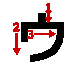
\includegraphics[trim= 00 05 00 00]{../share/katakana/us.pdf}
%\end{center}
\bigskip

\CharacterExplanation{us}{Write the first short stroke straight from up to
down. Then - and this is difficult, place the second stroke in the correct
distance from the first one. Luckily this is also a straight stroke from up to
down. }

\bigskip

Of course the perception changes if the character is written in a square.
Remember that it is better to write the character in a square, because the
correct spaces between the character and the frame also determinates its
beauty.

\bigskip

\CharacterExplanation{uss}{The first stroke in the frame is not difficult, as
mentioned before it goes from straight up to down. However the frame helps because now
we understood that it is centered. The second stroke becomes also easier in a
frame because it is written at the edge of the character. After some time and
experience this is better understood. The last stroke has to join the first and
second stroke. That is still difficult with or without a frame.}

\bigskip

%----------------------------------------------------------------------------
\subsection{Stroke Types}\jsubsec{筆画の種類}
% [o] LABEL
\label{sec:StrokeTypes}
\label{sec:Stroke}
\label{subsec:StrokeTypes}
% [o] INDEX
\ifor{stroke types}{筆画の種類}{ひっかくのしゅるい}{Strich Typen}
\ifor{stroke}{筆画}{ひっかく}{Strich}
\ifor{Hiragana}{平仮名}{ひらがな}{Hiragana}
\ifor{Kanji}{漢字}{かんじ}{Kanji}

In European language there is no idea to have different \textit{stroke} types
unless one enter the field of calligraphy. In Japanese there are different kind
of \textit{strokes}.  Most important for \hyperref[sec:Kanji]{Kanji}, second
important for \hyperref[sec:Hiragana]{Hiragana} and least important for
\textit{Katakana} since \textit{Katakana} is also used for a bold replacement.
Due to this fact the five different type of Japanese \textit{strokes}
({筆画の種類} {【ひっかくのしゅるい】}) will not repeated here. For now it is
perfectly fine to make all \textit{strokes} equally thick. 


